\documentclass[11pt]{article}
\usepackage[margin=1in]{geometry}
\usepackage{lmodern}
\usepackage[T1]{fontenc}
\usepackage{amsmath,amssymb}
\usepackage{booktabs}
\usepackage{graphicx}
\usepackage{caption}
\captionsetup{font=small,labelfont=bf}
\usepackage[numbers,sort&compress]{natbib}
\usepackage[colorlinks=true,citecolor=blue,urlcolor=blue,linkcolor=blue]{hyperref}
\usepackage{xcolor}
\setcitestyle{authoryear,round}
\setlength{\parskip}{0.3em}

\title{Predicting Feynman Periods with Graph Neural Networks\\[0.3em]\large Project Milestone}
\date{}

\begin{document}
\maketitle
\vspace{-3.5em}
\noindent\textbf{Members:} Ethan Katz, Evelyn Song, Colin McKhann\\
\textbf{Project Type:} Real-world applications of GNNs

\section*{1\quad Problem and Motivation}

The primitive contribution to the $\beta$ function of $\phi^4$-theory is a sum over Feynman periods,
\begin{equation*}
\mathcal{P}(G) = \int_{\alpha_e>0} \prod_{e\in E} d\alpha_e\,
\frac{\delta\big(1-\sum_{e\in E}\alpha_e\big)}{\psi_G(\alpha)^2},\qquad
\psi_G(\alpha)=\sum_{T\text{ spanning tree}}\ \prod_{e\notin T}\alpha_e ,
\end{equation*}
one per primitive (subdivergence-free) graph $G$. The number of graphs grows factorially with the
loop number $L$, and each period is an expensive numerical integral, so a cheap and accurate
predictor of $\mathcal{P}(G)$ from the graph alone would directly reduce the cost of high-order QFT
calculations. \citet{balduf2024predicting} showed that structural invariants (notably the
Hepp bound, Martin invariants and cycle/cut counts) predict periods well, but the strongest of
these are themselves costly to compute, and their GNNs, which started from arbitrary vertex
labels, never beat linear regression. Our project asks whether message-passing GNNs, given
\emph{cheap structural node features}, can learn periods from graph structure alone.

\paragraph{Milestone summary.} We built a complete, reproducible pipeline (download $\to$ parse
$\to$ PyG \texttt{Data} $\to$ grouped splits $\to$ training/evaluation of GCN, GraphSAGE and GIN
$\to$ non-GNN baselines), trained 48 GNN models (3 architectures $\times$ 8 node-feature sets
$\times$ 2 seeds) on all 92{,}680 primitive graphs with $3\le L\le 12$, and ran the ablation of our
proposed novelty: structural node features versus constant or arbitrary features.
\RESULTSUMMARY

\section*{2\quad Dataset and Processing}

\paragraph{Source.} We use the public dataset of \citet{balduf2024dataset} (Borealis Dataverse,
doi:10.5683/SP3/NLEDGH, CC-BY 4.0), which accompanies \citet{balduf2024predicting} and
\citet{balduf2023statistics}. File \texttt{periods\_L.csv} lists one graph per line, with its
numerical period, its uncertainty, the Hepp bound and further invariants. The dataset is
\emph{complete} up to $L=13$ and a non-uniform sample for $14\le L\le 18$.

\paragraph{Graph representation.} Each row gives the \emph{completion} of a Feynman graph: the
graph obtained by joining the four external legs to one new vertex. Completions are simple
4-regular graphs with $L+2$ vertices and $2(L+2)$ edges, and all decompletions of a completion share
the same period, so the completion is the natural (and non-redundant) input. We parse the
edge-list column into an undirected \texttt{edge\_index}, assert 4-regularity, and use
$y=\log\mathcal{P}(G)$ as the regression target, since periods span several orders of magnitude
(Fig.~\ref{fig:data}a) and errors in $\log\mathcal{P}$ are relative errors in $\mathcal{P}$. For
the milestone we use $3\le L\le 12$ (Table~\ref{tab:data}); $L=12$ alone contributes 81{,}305
graphs of 14 vertices and 28 edges each. The $L=13$ file (94\,MB compressed, $\approx$0.9M graphs)
is the next step.

\begin{table}[h]
\centering\small
\caption{Graphs per loop order used in the milestone (all primitive $\phi^4$ completions).}
\label{tab:data}
\begin{tabular}{lcccccccccc|c}
\toprule
$L$ & 3 & 4 & 5 & 6 & 7 & 8 & 9 & 10 & 11 & 12 & total\\
\midrule
graphs & 1 & 1 & 2 & 5 & 14 & 49 & 227 & 1{,}354 & 9{,}722 & 81{,}305 & 92{,}680\\
\bottomrule
\end{tabular}
\end{table}

\paragraph{Leakage-free splits.} Many distinct graphs have \emph{provably identical} periods
(product, twist, Fourier and planar-duality symmetries), and the dataset stores them with
bit-identical values. A random split would therefore place a graph in the test set whose exact
label appears in training. We instead split \emph{groups} of identical period values 80/10/10 into
train/validation/test within every loop order, giving 74{,}202 / 9{,}145 / 9{,}333 graphs. The test set
is dominated by $L=11,12$, where the problem is hardest.

\begin{figure}[t]
\centering
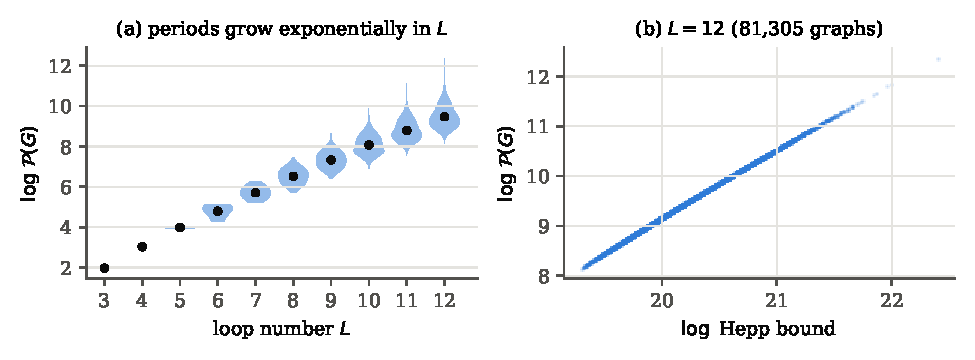
\includegraphics[width=\linewidth]{../figures/data_overview.pdf}
\vspace{-1.5em}
\caption{(a) Distribution of $\log\mathcal{P}$ per loop order: the loop number explains the mean,
but within one $L$ periods still span more than an order of magnitude (a factor of $\sim$50 at
$L=12$), and this within-loop variation is what a model must learn. (b) At $L=12$ the (expensive) Hepp bound is almost a deterministic function of the period,
as observed by \citet{balduf2024predicting}.}
\label{fig:data}
\end{figure}

\section*{3\quad Model Design and Metrics}

\paragraph{Architectures.} All GNNs share one skeleton so that only the message-passing operator
varies: a linear node encoder, $K=4$ message-passing layers of width 64 (each followed by
BatchNorm, ReLU and a residual connection), a readout concatenating sum- and mean-pooling, and a
two-layer MLP head. The operators are GCN \citep{kipf2017gcn},
$H^{(l+1)}=\sigma(\tilde D^{-1/2}\tilde A\tilde D^{-1/2}H^{(l)}W^{(l)})$; GraphSAGE
\citep{hamilton2017sage}, $h_v^{(l+1)}=\sigma(W^{(l)}[h_v^{(l)}\,\|\,\mathrm{mean}_{u\in N(v)}h_u^{(l)}])$;
and GIN \citep{xu2019gin}, $h_v^{(l+1)}=\mathrm{MLP}^{(l)}((1+\epsilon^{(l)})h_v^{(l)}+\sum_{u\in N(v)}h_u^{(l)})$.
Models are trained with AdamW (lr $2\cdot10^{-3}$, cosine schedule, batch 256, 40 epochs) on the
MSE of the standardized target; the checkpoint with the lowest validation MAE is evaluated on
test. For constant features we drop BatchNorm (\texttt{--norm none}): with identical inputs every
node embedding is identical, BatchNorm's running variance collapses to zero and evaluation-mode
outputs diverge, which is what happened in our first attempt. Each run takes $\approx$5 minutes on one CPU core of an M1 Max laptop.

\paragraph{Why node features matter here.} Every completed $\phi^4$ graph is 4-regular. With
constant input features, 1-WL colour refinement assigns every vertex of every such graph the same
colour at every iteration, and message-passing GNNs are at most as expressive as 1-WL
\citep{xu2019gin}. A GNN with constant features can therefore compute nothing but a function of
the number of vertices, i.e.\ of $L$: it can do no better than the per-loop mean, which is exactly
the linear-regression baseline that earlier NNs failed to beat. This makes the input features,
not the architecture, the crux of the problem, and motivates our ablation:
\begin{itemize}\setlength\itemsep{0em}
\item \textbf{constant}: $x_v=1$ (structure-free control);
\item \textbf{random label}: one-hot of a uniformly random vertex permutation, resampled at every
forward pass, i.e.\ genuinely arbitrary vertex labels as used by earlier GNNs;
\item \textbf{canonical label}: one-hot of the vertex label \emph{as stored in the dataset}. These
labels are nauty's canonical form, so together with the edges they identify the graph up to
isomorphism. This is not equivariant, but it is a strong structural signal rather than noise (see
Section~4);
\item \textbf{random (RNI)}: 8 i.i.d.\ Gaussian features resampled every forward pass
\citep{sato2021rni,abboud2021rni};
\item \textbf{cycle participation} (ours): $c_k(v)=\#\{\text{simple cycles of length }k\text{ through }v\}$
for $k=3,\dots,8$, as $\log(1+c_k)$. We enumerate cycles exactly with a Numba-compiled DFS; summing
$c_k(v)/k$ over $v$ reproduces the dataset's graph-level cycle counts exactly, which we use as a
correctness check;
\item \textbf{LapPE} (ours): the 8 lowest non-trivial eigenvectors of the normalized Laplacian
\citep{dwivedi2023benchmarking}, with random sign flips during training;
\item \textbf{RWSE}: random-walk return probabilities $(P^t)_{vv}$, $t=1..12$
\citep{dwivedi2022rwse}, a cheap proxy that mixes cycles with backtracking walks;
\item combinations \textbf{cycle+LapPE} and \textbf{cycle+LapPE+RWSE}.
\end{itemize}
All structural features are computed in $\approx$45\,s for the whole dataset on one core, many
orders of magnitude cheaper than computing the periods themselves.

\paragraph{Non-GNN baselines.} (i) Linear regression of $\log\mathcal{P}$ on $L$; (ii) ridge
regression on one-hot($L$) plus $\log(1+\text{graph-level cycle counts})$, which uses the
\emph{same} information as our cycle features but pools it before learning, isolating the value of
message passing; (iii) ridge on one-hot($L$) plus $\log$ Hepp bound, reported as a reference only,
because the Hepp bound is itself an expensive combinatorial quantity (a sum over all edge
orderings).

\paragraph{Metrics.} We report (a) the \textbf{mean relative error} $\frac1N\sum|\hat{\mathcal P}-\mathcal P|/\mathcal P$
(the metric of \citealp{balduf2024predicting}); (b) the MAE of $\log\mathcal{P}$; and (c) the
\textbf{within-loop $R^2$}, $1-\sum(\hat y-y)^2/\sum(y-\bar y_{L})^2$, where $\bar y_L$ is the mean
true $\log\mathcal{P}$ of the graph's loop order. Ordinary $R^2$ is inflated by the trivial
dependence on $L$; within-loop $R^2$ measures how much of the genuinely hard, within-$L$ variance is
explained (0 for the linear-in-$L$ baseline).

\section*{4\quad Preliminary Results}

\RESULTS

\section*{5\quad Next Steps}

\NEXTSTEPS

\bibliographystyle{plainnat}
\begin{thebibliography}{99}\small
\bibitem[Abboud et~al.(2021)]{abboud2021rni}
R.~Abboud, \.I.~\.I.~Ceylan, M.~Grohe, and T.~Lukasiewicz.
\newblock The surprising power of graph neural networks with random node initialization.
\newblock In \emph{IJCAI}, 2021.

\bibitem[Balduf(2023)]{balduf2023statistics}
P.-H.~Balduf.
\newblock Statistics of {F}eynman amplitudes in $\phi^4$-theory.
\newblock \emph{JHEP}, 11:160, 2023. arXiv:2305.13506.

\bibitem[Balduf and Shaban(2024a)]{balduf2024predicting}
P.-H.~Balduf and K.~Shaban.
\newblock Predicting {F}eynman periods in $\phi^4$-theory.
\newblock arXiv:2403.16217, 2024.

\bibitem[Balduf and Shaban(2024b)]{balduf2024dataset}
P.-H.~Balduf and K.~Shaban.
\newblock Feynman periods in $\phi^4$-theory [dataset].
\newblock Borealis Dataverse, 2024. \href{https://doi.org/10.5683/SP3/NLEDGH}{doi:10.5683/SP3/NLEDGH}.

\bibitem[Dwivedi et~al.(2022)]{dwivedi2022rwse}
V.~P.~Dwivedi, A.~T.~Luu, T.~Laurent, Y.~Bengio, and X.~Bresson.
\newblock Graph neural networks with learnable structural and positional representations.
\newblock In \emph{ICLR}, 2022.

\bibitem[Dwivedi et~al.(2023)]{dwivedi2023benchmarking}
V.~P.~Dwivedi, C.~K.~Joshi, A.~T.~Luu, T.~Laurent, Y.~Bengio, and X.~Bresson.
\newblock Benchmarking graph neural networks.
\newblock \emph{JMLR}, 24(43):1--48, 2023.

\bibitem[Hamilton et~al.(2017)]{hamilton2017sage}
W.~L.~Hamilton, R.~Ying, and J.~Leskovec.
\newblock Inductive representation learning on large graphs.
\newblock In \emph{NeurIPS}, 2017.

\bibitem[Kipf and Welling(2017)]{kipf2017gcn}
T.~N.~Kipf and M.~Welling.
\newblock Semi-supervised classification with graph convolutional networks.
\newblock In \emph{ICLR}, 2017.

\bibitem[Sato et~al.(2021)]{sato2021rni}
R.~Sato, M.~Yamada, and H.~Kashima.
\newblock Random features strengthen graph neural networks.
\newblock In \emph{SDM}, 2021.

\bibitem[Xu et~al.(2019)]{xu2019gin}
K.~Xu, W.~Hu, J.~Leskovec, and S.~Jegelka.
\newblock How powerful are graph neural networks?
\newblock In \emph{ICLR}, 2019.
\end{thebibliography}

\end{document}
